\documentclass[handout]{ximera}
%handout:  for handout version with no solutions or instructor notes
%handout,instructornotes:  for instructor version with just problems and notes, no solutions
%noinstructornotes:  shows only problem and solutions

%% handout
%% space
%% newpage
%% numbers
%% nooutcomes

%I added the commands here so that I would't have to keep looking them up
%\newcommand{\RR}{\mathbb R}
%\renewcommand{\d}{\,d}
%\newcommand{\dd}[2][]{\frac{d #1}{d #2}}
%\renewcommand{\l}{\ell}
%\newcommand{\ddx}{\frac{d}{dx}}
%\everymath{\displaystyle}
%\newcommand{\dfn}{\textbf}
%\newcommand{\eval}[1]{\bigg[ #1 \bigg]}

%\begin{image}
%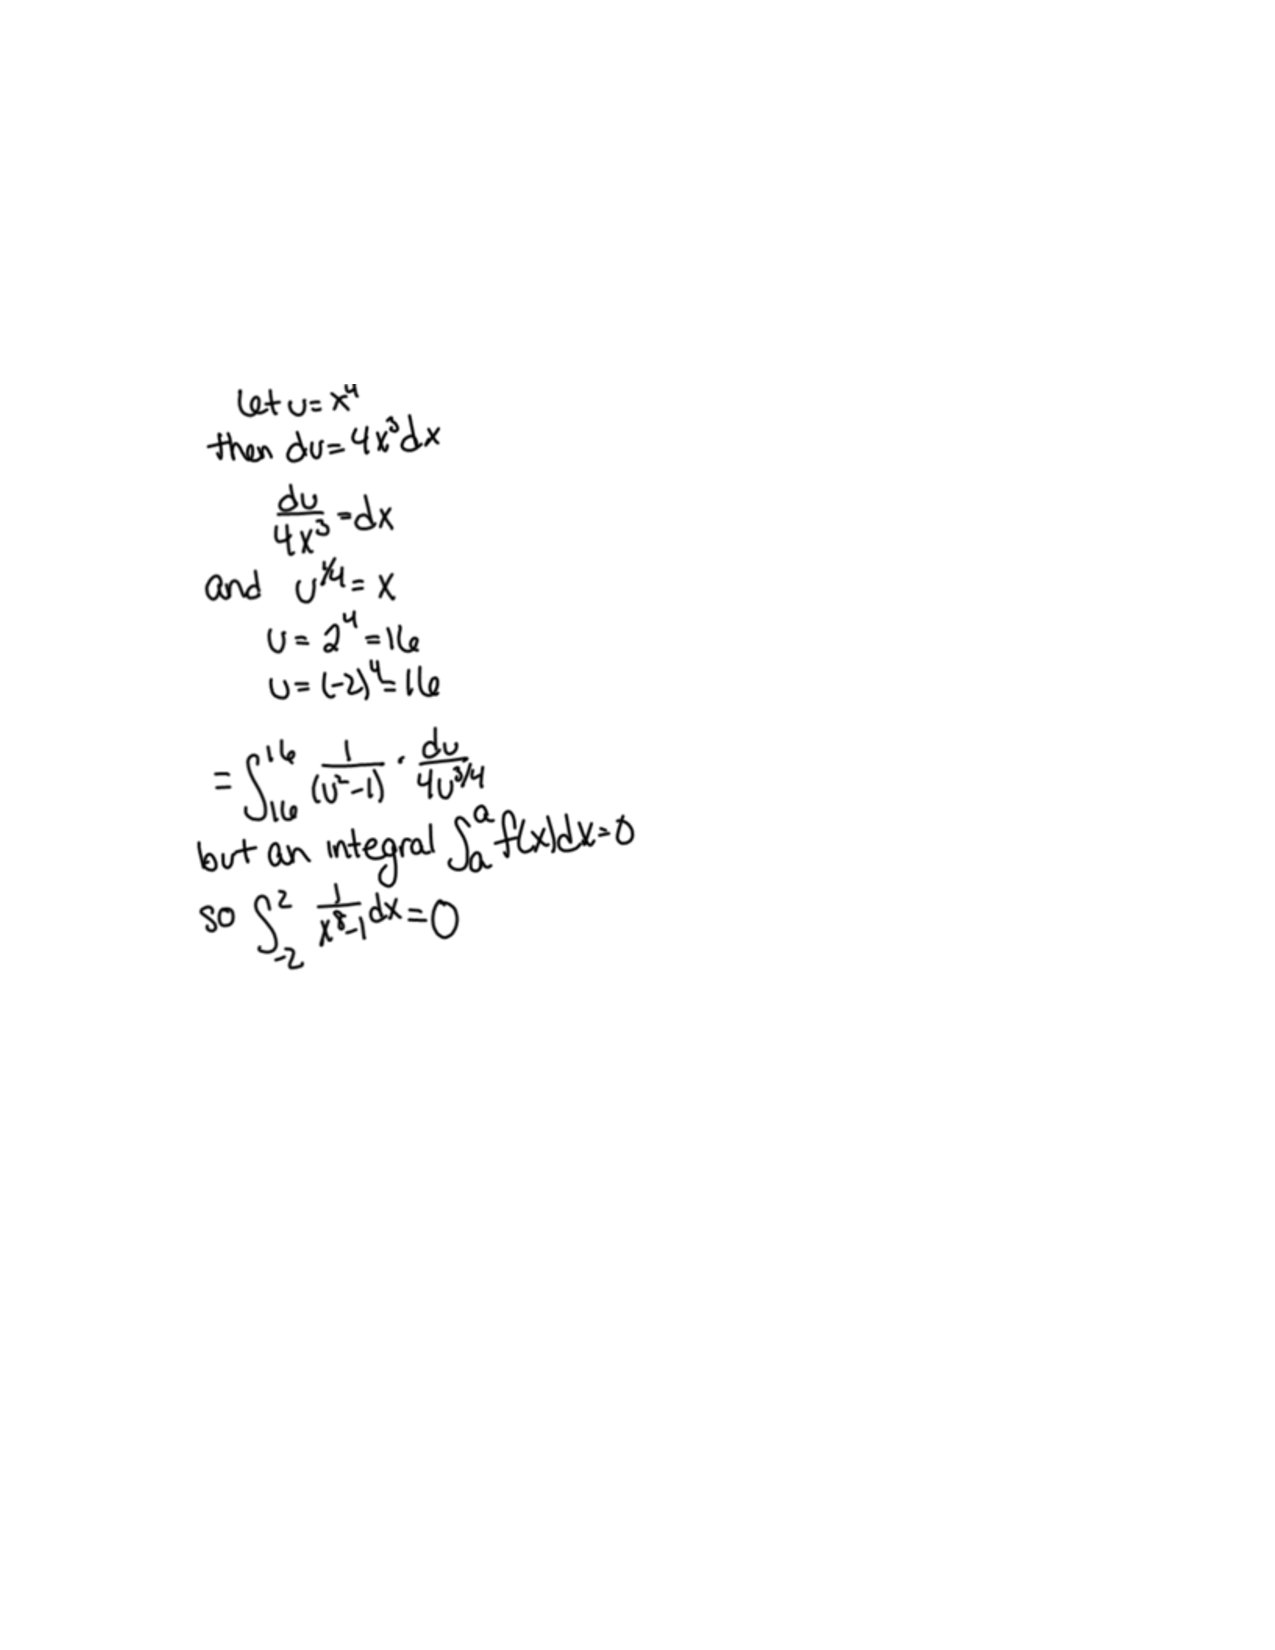
\includegraphics[trim= 170 420 250 180]{Figure1.pdf}
%\end{image}

%add a ``.'' below when used in a specific directory.
\newcommand{\RR}{\mathbb R}
\renewcommand{\d}{\,d}
\newcommand{\dd}[2][]{\frac{d #1}{d #2}}
\renewcommand{\l}{\ell}
\newcommand{\ddx}{\frac{d}{dx}}
\newcommand{\dfn}{\textbf}
\newcommand{\eval}[1]{\bigg[ #1 \bigg]}

\usepackage{multicol}

\renewenvironment{freeResponse}{
\ifhandout\setbox0\vbox\bgroup\else
\begin{trivlist}\item[\hskip \labelsep\bfseries Solution:\hspace{2ex}]
\fi}
{\ifhandout\egroup\else
\end{trivlist}
\fi} %% we can turn off input when making a master document

\title{Recitation 28: Cross Products and Lines and Curves in Space}  

\begin{document}
\begin{abstract}		\end{abstract}
\maketitle



\section{Warm up:}



If $\vec{a}$, $\vec{b}$, and $\vec{c}$ are vectors in $3$-space $\mathbb{R}^3$, which of the following make sense?
	\begin{multicols}{3}
	\begin{enumerate}
	\item  $(\vec{a} \cdot \vec{b}) \cdot \vec{c}$
	\item  $(\vec{a} \cdot \vec{b})\vec{c}$
	\item  $(\vec{a} \times \vec{b}) \cdot \vec{c}$
	\item  $(\vec{a} \cdot \vec{b}) + \vec{c}$
	\item  $(\vec{a} \times \vec{b}) + \vec{c}$
	\item  $\vec{a} \cdot (\vec{b} + \vec{c})$
	\item  $\vec{a} \cdot (\vec{b} \times \vec{c})$
	\item  $\vec{a} \times (\vec{b} \cdot \vec{c})$
	\item  $(\vec{a} \times \vec{b}) \vec{c}$
	\end{enumerate}
	\end{multicols}
	
	\begin{freeResponse}
	\begin{enumerate}
	\item  Since $\vec{a} \cdot \vec{b}$ is a scalar, $(\vec{a} \cdot \vec{b}) \cdot \vec{c}$ does \dfn{not} make sense.
	\item  Now since $\vec{a} \cdot \vec{b}$ is a scalar, $(\vec{a} \cdot \vec{b})\vec{c}$ \dfn{does} make sense as regular scalar multiplication.
	\item  Since $\vec{a} \times \vec{b}$ is a vector, $(\vec{a} \times \vec{b}) \cdot \vec{c}$ \dfn{does} make sense.
	\item  This is of the form ``scalar + vector'', which does \dfn{not} make sense.
	\item  Since $\vec{a} \times \vec{b}$ is a vector, $(\vec{a} \times \vec{b}) + \vec{c}$ \dfn{does} make sense.
	\item  This is of the form ``vector $\cdot$ vector'', which \dfn{does} make sense.
	\item  This is also of the form ``vector $\cdot$ vector'', which \dfn{does} make sense.
	\item  This is of the form ``vector $\times$ scalar'', which does \dfn{not} make sense.
	\item  Since $\vec{a} \times \vec{b}$ is a vector, this does \dfn{not} make sense.
	\end{enumerate}
	\end{freeResponse}
	
\begin{instructorNotes}
This problem can be split up among the groups if the instructor likes (with maybe 3 or so per group).  
\end{instructorNotes}






\section{Group work:}

%problem 1
\begin{problem}
Given three dimensional vectors $\vec{u}$, $\vec{v}$, and $\vec{w}$, use dot product or cross product notation to describe the following vectors:
	\begin{enumerate}
	\item  The vector projection of $\vec{w}$ onto $\vec{u}$.
	
	\item  A vector orthogonal to both $\vec{u}$ and $\vec{v}$.
	
	\item  A vector with the length of $\vec{v}$ and the direction of $\vec{w}$.  
	
	\item  A vector orthogonal to $\vec{u} \times \vec{v}$ and $\vec{w}$.
	\end{enumerate}
	
	\begin{freeResponse}
	\begin{enumerate}
	\item  This is the definition of vector projections.
		\[
		\text{proj}_u w = \boxed{\left( \frac{\vec{u} \cdot \vec{w}}{\vec{u} \cdot \vec{u}} \right) \vec{u}}
		\]
	
	\item  There are many such vectors, but one of them is
		\[
		\boxed{\vec{u} \times \vec{v}}
		\]
	
	\item  Note that $|\vec{v}|^2 = \vec{v} \cdot \vec{v}$ so that $|\vec{v}|=\sqrt{\vec{v} \cdot \vec{v}}$. 
		\[
		| \vec{v} | \left( \frac{\vec{w}}{| \vec{w} |} \right) = \boxed{ \frac{\sqrt{\vec{v} \cdot \vec{v}}}{\sqrt{\vec{w} \cdot \vec{w}}} \vec{w}}
		\]
	
	\item  
		\[
		\boxed{(\vec{u} \times \vec{v}) \times \vec{w}}
		\]
	\end{enumerate}
	\end{freeResponse}
	
\end{problem}

\begin{instructorNotes}
This problem and the Warm-up are meant to force the students to make sense of scalar vs. vector quantities, as well as what quantities the dot and cross products produce.
\end{instructorNotes}







%problem 2
\begin{problem} 
Let $\vec{u} =\langle 5,-1,8 \rangle$ and $\vec{v} = \langle -2,10,5 \rangle$.
\begin{enumerate}
\item Find a vector that is perpendicular to both $\vec{u}$ and $\vec{v}$.  
\item Verify that your answer is perpendicular to both $\vec{u}$ and $\vec{v}$
\item Find a vector of length 7 perpendicular to both $\vec{u}$ and $\vec{c}$.
\end{enumerate}

	\begin{freeResponse}
	\begin{enumerate}
	\item 
	Let $\vec{u} = \langle 5,-1,8 \rangle$ and $\vec{v} = \langle -2,10,5 \rangle$.
	Then a vector which is perpendicular to both $\vec{u}$ and $\vec{v}$ is $\vec{w} := \vec{u} \times \vec{v}$.  
	So we calculate
		\begin{align*}
		\vec{w} = \vec{u} \times \vec{v} = 
		\begin{vmatrix}
		\hat{\imath}	&	\hat{\jmath}	&	\hat{k}	\\
		5		&	-1		&	8		\\
		-2		&	10		&	5		\\
		\end{vmatrix}
		&= (-5 - 80) \hat{\imath} - (25 + 16) \hat{\jmath} + (50 - 2) \hat{k}  \\
		&= -85 \hat{\imath} -41 \hat{\jmath} + 48 \hat{k}
		\end{align*}
		
	\item To verify perpendicularity, we take the dot product.\\
	\[
	\vec{u} \cdot \vec{w} = \langle 5,-1,8 \rangle \cdot \langle -85, -41, 48 \rangle = 5(-85)-1(-41)+8(48) = -425 +41 + 384 = 0 
	\]
	\[
	\vec{v} \cdot \vec{w} = \langle -2,10,5 \rangle \cdot \langle -85, -41, 48 \rangle = -2(-85) +10(-41)+5(48) = 170 -410 + 240 = 0 \\
	\]	
		
	\item	
	A unit vector in the same direction as $\vec{w}$ is
		\[
		\frac{\vec{w}}{| \vec{w} |}
		= \frac{1}{\sqrt{(-85)^2 + (-41)^2 + 48^2}} \vec{w} = \frac{1}{\sqrt{11210}} \vec{w}.
		\]
	Therefore, a vector with a magnitude of $7$ in the same direction as $\vec{w}$ is
		\[
		\vec{t} = \frac{7}{| \vec{w} |} \vec{w} = \boxed{\frac{7}{\sqrt{11210}} \langle -85,-41,48 \rangle}
		\]
		
		\end{enumerate}
		
	\end{freeResponse}
		
\end{problem}

\begin{instructorNotes}
Using cross product to find perpendicular vectors. 
\end{instructorNotes}




%problem3
\begin{problem}
Find the area of the triangle in $\mathbb{R}^3$ with vertices at $P(2, -1, 0)$, $Q(1, 1, 4)$ and $R(2, -1, 6)$. 
	\begin{freeResponse}
	The area of the triangle is $\frac{1}{2} | \vec{PQ} \times \vec{PR}|$. 
	\begin{align*}
	\vec{PR} &= \langle 2, -1, 6 \rangle - \langle 2, -1, 0 \rangle = \langle 0, 0, 6 \rangle, \\
	\vec{PQ} &= \langle 1, 1, 4, \rangle - \langle 2, -1, 0 \rangle = \langle -1, 2, 4 \rangle.
	\end{align*}
	So 
	\begin{align*}
	\vec{PQ} \times \vec{PR} &= (-\vec{i} +2\vec{j} +4\vec{k})\times 6\vec{k} = - (\vec{i}\times \vec{k}) +2 (\vec{j} \times \vec{k}) +24 (\vec{k}\times \vec{k}) \\ &= - (-\vec{j}) + 2 \vec{i} + 0 = \langle 2, 1, 0 \rangle.
	\end{align*}
	The area of the triangle is $\frac{1}{2} \sqrt{2^2+1^2+0^2} = \frac{\sqrt{5}}{2}$. 
	\end{freeResponse}
		
\end{problem}

\begin{instructorNotes}
Students should know that we can find the areas of triangles and parallelograms in $\mathbb{R}^3$ by using the cross product.
\end{instructorNotes}

\begin{problem}
Find a vector-valued function for the line segment connecting the points $P = (-3,7,6)$ and $Q = (5,-4,7)$ in such a way that the value at $t=0$ is $P$ and the value at $t=1$ is $Q$.  
Also, find the point two-thirds of the way from $P$ to $Q$.
	\begin{freeResponse}
	The line segment $\vec{r}(t)$ from $P$ to $Q$ is 
		\begin{align*}
		\vec{r}(t) &= (1-t)P + tQ  \\
		&= (1-t) \langle -3,7,6 \rangle + t \langle 5,-4,7 \rangle  \\
		&= \boxed{\langle -3 + 8t, 7 - 11t, 6 + t \rangle \quad \text{for }0 \leq t \leq 1}.
		\end{align*}
	The point two-thirds of the way from $P$ to $Q$ is
		\begin{align*}
		\vec{r} \left( \frac{2}{3} \right)
		&= \left\langle -3 + 8 \left( \frac{2}{3} \right), 7 - 11\left( \frac{2}{3} \right), 6 + \frac{2}{3} \right\rangle  \\
		&= \boxed{\left\langle \frac{7}{3} , - \frac{1}{3}, \frac{20}{3} \right\rangle}
		\end{align*}
	\end{freeResponse}
	
\begin{instructorNotes}
A common mistake is to forget the domain of $t$. 
\end{instructorNotes}
\end{problem}


%problem 1
\begin{problem}
Find a vector-valued function for the line through the point $(1,-2,3)$ that is perpendicular to the lines
	\[
	\vec{r}_1(t) = \langle 7,8,-2 \rangle + t \langle 3,5,7 \rangle 
	\quad \text{and} \quad 
	\vec{r}_2(s) = \langle 4,-3,-7 \rangle + s \langle 4,9,-1 \rangle
	\]
	\begin{freeResponse}
	Let $\vec{v}_1 = \langle 3,5,7 \rangle$ and $\vec{v}_2 = \langle 4,9,-1 \rangle$.
	Then $\vec{v}_1$ is parallel to the line $\vec{r}_1$, and similarly for $\vec{v}_2$ and $\vec{r}_2$.  
	So a vector perpendicular to both of the lines $\vec{r}_1$ and $\vec{r}_2$ is
		\begin{align*}
		\vec{n} = \vec{v}_1 \times \vec{v}_2  
		&= \begin{vmatrix}
		\hat{\imath}	&	\hat{\jmath}	&	\hat{k}	\\
		3		&	5		&	7		\\
		4		&	9		&	-1		\\
		\end{vmatrix}  \\
		&= (-5-63)\hat{\imath} - (-3-28)\hat{\jmath} + (27-20)\hat{k}  \\
		&= \langle -68, 31, 7 \rangle.
		\end{align*}
	So the equation of the line through $(1,-2,3)$ and perpendicular to both $\vec{r}_1$ and $\vec{r}_2$ is
		\begin{align*}
		\vec{r}_3(t) &= \langle 1,-2,3 \rangle + t \langle -68,31,7 \rangle  \\
		&= \boxed{\langle 1-68t,-2+31t,3+7t \rangle \quad \text{for }-\infty < t < \infty}
		\end{align*}
	\end{freeResponse}
	
\end{problem}

\begin{instructorNotes}

\end{instructorNotes}















%problem 3
\begin{problem}
Show that the curve $\vec{r} = \langle t \cos t, t \sin t, t \rangle$ lies completely on the cone $z^2 = x^2 + y^2$.  
	\begin{freeResponse}
	We just need to check that the components of $\vec{r}$ satisfies the given equation.  
	So we compute
		\begin{align*}
		x^2 + y^2 &= (t \cos t)^2 + (t \sin t)^2  \\
		&= t^2 \cos^2 t + t^2 \sin^2 t  \\
		&= t^2 (\cos^2 t + \sin^2 t)  \\
		&= t^2  \\
		&= z^2.
		\end{align*}
	\end{freeResponse}

\end{problem}

\begin{instructorNotes}

\end{instructorNotes}




\section{Challenge Problems}

%problem 2
\begin{problem}
Find the distance from the point $P(-1,4,3)$ to the line $\langle 8+t,3-3t,-26t \rangle$.  {\it Hint: The distance from the point to the line is the distance from the point $P$ and the closest point on the line.}
	\begin{freeResponse}
	Let $P = (-1,4,3)$ and, for any time $t$, let $Q(t) = (8+t,3-3t,-26t)$.  
	Then the distance from $P$ to $Q(t)$ is given by
		\begin{align*}
		D(t) &=
		\sqrt{(8+t - (-1))^2 + (3-3t -4)^2 + (-26t-3)^2}  \\
		&= \sqrt{(9+t)^2 + (-1-3t)^2 + (-3-26t)^2}.
		\end{align*}
	Instead of minimizing the distance $D(t)$, we will minimized the square of the distance $D^2(t)$, which leads to the same point.  
	So
		\[
		D^2(t) = (9+t)^2 + (-1-3t)^2 + (-3-26t)^2.
		\]
	To find the minimum of this function, we differentiate and find critical points
		\begin{align*}
		\frac{\d}{\d t} D^2(t) &= 2(9+t) + 2(-1-3t)(-3) + 2(-3-26t)(-26)  \\
		&= (18 + 2t) + (6 + 18t) + (156 + 1352t)  \\
		&= 180 + 1372t := 0  \\
		\Longrightarrow \qquad t &= - \frac{180}{1372} = - \frac{45}{343}.
		\end{align*}
	Since there is exactly one critical point and since the second derivative is positive (it is the constant $1372$), this value of $t$ gives an absolute minimum.
	Therefore, the distance from $P$ to the line is
		\[
		\boxed{\sqrt{\left( 9-\frac{45}{343} \right)^2 + \left(-1-3\left( - \frac{45}{343} \right) \right)^2 + \left(-3-26\left( - \frac{45}{343} \right) \right)^2}}
		\]
	\end{freeResponse}
 \end{problem}

\begin{instructorNotes}

\end{instructorNotes}
 
 
 \newpage
%problem 4
\begin{problem}
Match each of the following curves to the corresponding vector-valued function.
	\begin{multicols}{3}
	\begin{enumerate}
	\item  $\langle 3, t^2,5 \rangle$
	\item  $\langle 3, t^2,t \rangle$
	\item  $\langle 3, \sin t , \cos t \rangle$
	\item  $\langle 3t,5 \sin t, 5\cos t \rangle$
	\item  $\langle \sin t, \cos t, 2 \cos t \rangle$
	\item  $\langle 2 \cos t, \sin t, \cos (3t) \rangle$
	\end{enumerate}
	\end{multicols}
	
	\begin{image}
	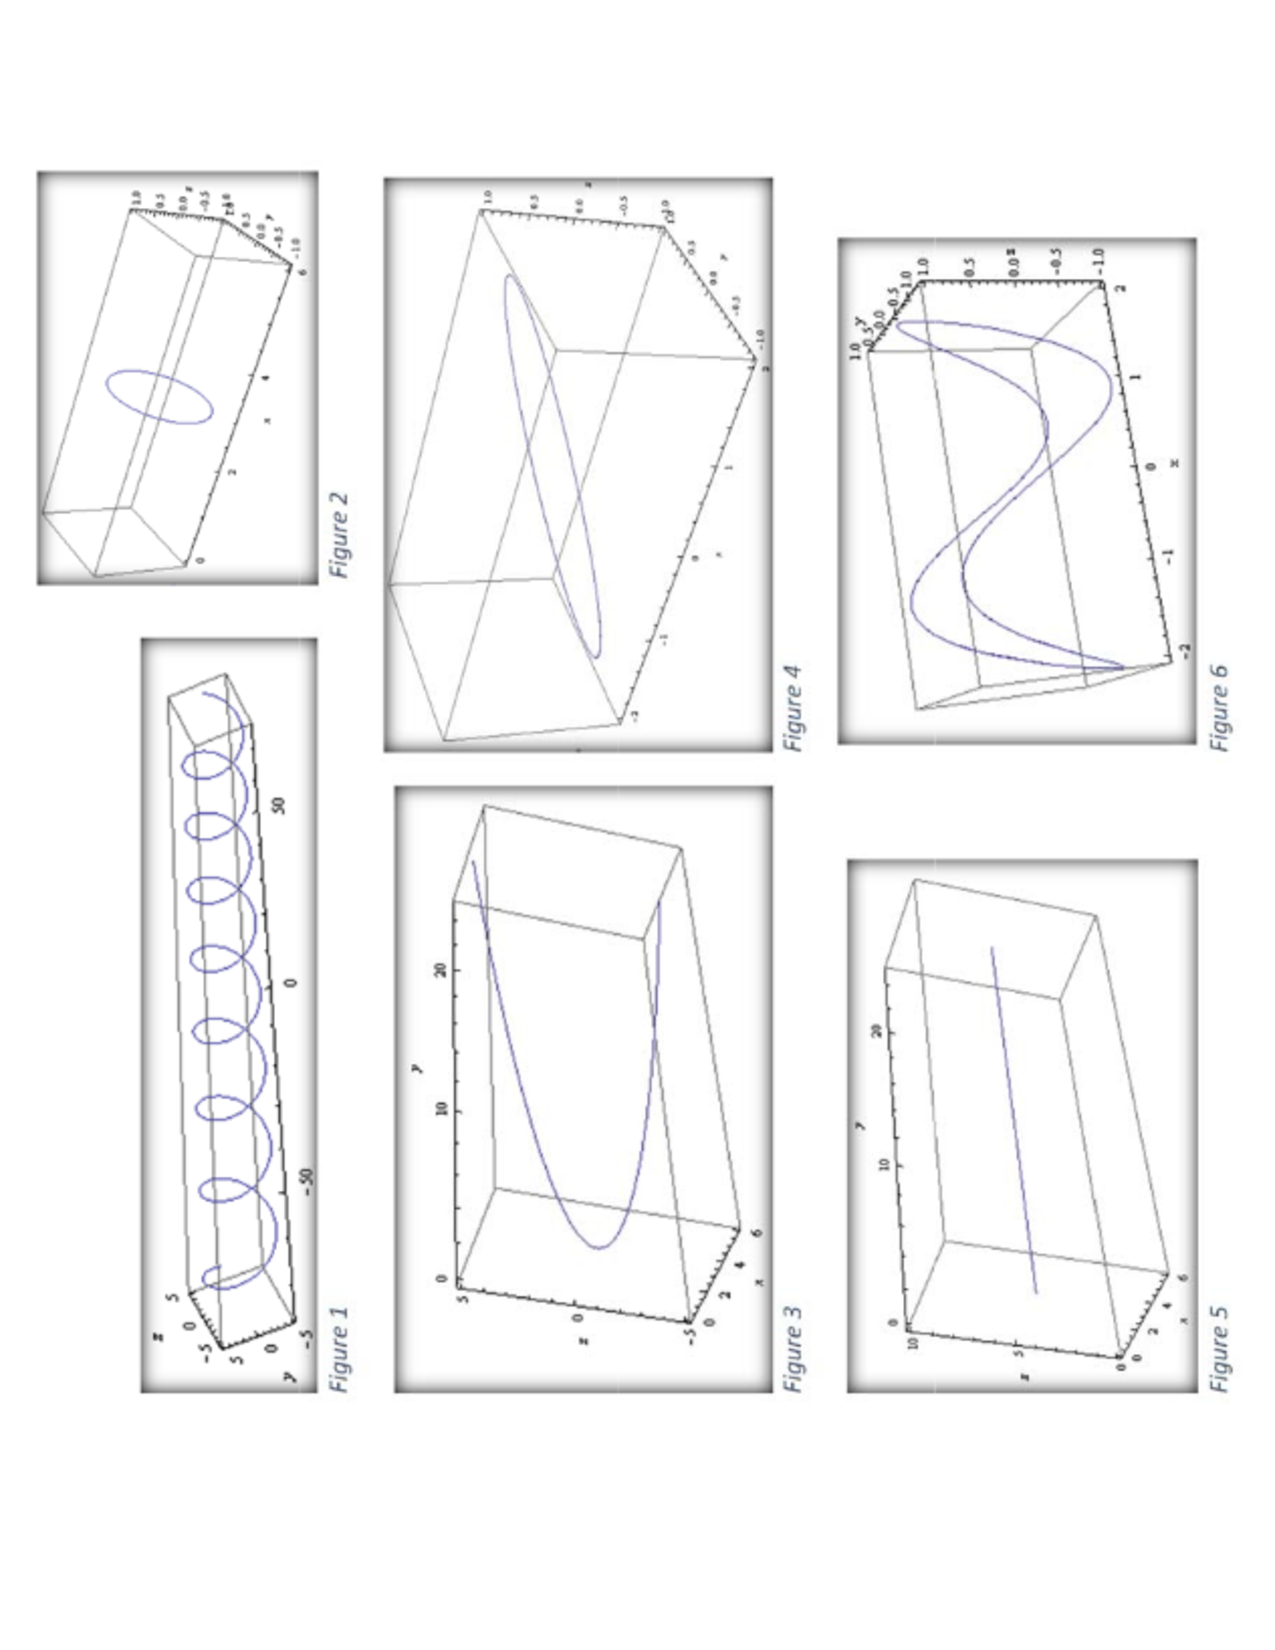
\includegraphics[angle=-89.99,trim= 40 120 0 120, scale=0.65]{Figure12-5-1.pdf}
	\end{image}
	
	\begin{freeResponse}
	\begin{enumerate}
	\item  {\bf Figure 5}.  This is a line with both $x$ and $z$ held fixed.
	
	\item  {\bf Figure 3}.  This is a parabola parallel to the $yz$-plane at $x=3$. 
	
	\item  {\bf Figure 2}.  This is a circle of radius $1$ in the plane $x=3$.  
	
	\item  {\bf Figure 1}.  The $x$-component is linear, while the projection onto the $yz$-plane is a circle of radius $5$.  
	So this looks like a ``spring''.
	
	\item  {\bf Figure 4}.  This is a circle with radius $1$ when projected onto the $xy$-plane.
	
	\item  {\bf Figure 6}.  This one is tricky.  Maybe the best way to spot it is that it is an ellipse when projected onto the $xy$-plane, while the $z$-component varies between $-1$ and $1$.
	
	\end{enumerate}
	\end{freeResponse}

\end{problem}

\begin{instructorNotes}

\end{instructorNotes}





		












	
	
	
	
	
	
	
	
	

	










								
				
				
	














\end{document} 


















